\documentclass[11pt]{article}

\usepackage{amsmath,amsthm,amssymb}
\usepackage{hyperref}
\usepackage[margin=1in]{geometry}
\usepackage{graphicx}
\usepackage{enumerate}
\usepackage{caption}
\usepackage{subcaption}

\usepackage{multicol}

\theoremstyle{definition}
\newtheorem{thm}{Theorem}
\newtheorem{hyp}[thm]{Hypothesis}
\newtheorem{cor}[thm]{Corollary}
\newtheorem{lem}[thm]{Lemma}
\newtheorem{prop}[thm]{Proposition}
\newtheorem{rem}[thm]{Remark}
\numberwithin{equation}{section}
\numberwithin{thm}{section}

\DeclareMathOperator\erf{erf}



\newcommand{\winva}{{w_1^{-1}(a)}}
\newcommand{\winvb}{{w_1^{-1}(b)}}
\renewcommand{\a}{a}
\renewcommand{\b}{b}
\newcommand{\m}{m}
\newcommand{\mtwo}{1}

\usepackage{authblk}

\title{Periodic Traveling Waves in an Integro-Difference Equation With a Nonmonotone Growth Function and Strong Allee Effect}
\date{}
\author{Michael Nestor and Bingtuan Li
\thanks{M. Nestor's email is \href{mailto:mdnest01@gmail.com}{mdnest01@gmail.com}. B. Li was partially supported by the National Science Foundation under Grant DMS-1515875 and Grant DMS-1951482.}}

\affil{Department of Mathematics, University of Louisville, \newline Louisville, KY 40292.}


\begin{document}


\maketitle
\begin{abstract}
Sufficient conditions are derived for the existence of a periodic traveling wave with two intermediate wave speeds for an integro-difference equation with a piecewise constant growth function exhibiting a period-2 cycle and a strong Allee effect. The mean traveling wave speed is shown to be the spreading speed of 
of solutions with compactly supported initial data under appropriate conditions. Case studies are conducted for the Laplace kernel and uniform kernel.
\end{abstract}


{\bf Key words:} Integro-difference equation, period two cycle, Allee effect, periodic traveling wave.
\newline


{\bf AMS Subject Classification:} 92D40, 92D25.



\section{Introduction}

Integro-difference equations in the form 
\begin{align}\label{q}
u_{n+1}(x)\;=\;Q[u_n](x)\;:=(k*(g\circ u_n))(x)\;=\,\int^{\infty}_{-\infty}k(x-y)\,g\big(u_n(y)\big)\,\mathrm{d}y,
\end{align}
are of great interest in the studies of invasions of populations with discrete generations and separate growth and dispersal stages. They have been used to predict changes in gene frequency \cite{lui82a, lui82b, lui83, slatkin, w78}, and applied to ecological problems~\cite{hh, ks, kot89, kot92, kotbook, lut, nkl,otto}. Previous rigorous studies on integro-difference equations have assumed that the growth function is nondecreasing~\cite{w78, wein82}, or  is nonmonotone without Allee effect~\cite{lui83, wang}. The results show existence of constant spreading speeds and travelng waves with fixed shapes and speeds.   Sullivan et al. ~\cite{pnas} demonstrated numerically  that an integro-difference equation with a nonmonotone growth function exhibiting  a strong Allee effect can generate traveling waves with fluctuating speeds, and Otto~\cite{otto} showed  that such an equation can have robust non-spreading solutions. In this paper we give conditions for the existence of a periodic traveling wave with two intermediate speeds for 
an integro-difference equation with a piecewise constant growth function that exhibits a strong Allee effect and a period-2 cycle. 

Piecewise constant growth functions have been used in the studies of integro-difference equations; see for example~\cite{kot1, lut, otto,  pnas}. Such an equation 
is analytically tractable and it can provide specific insights into the dynamics of solutions.  For the piecewise constant growth function
\begin{equation} \label{g0}
g(u) = \begin{cases}
0, & \text{if } u < \a, \\
1, & \text{if } u \geq \a,
\end{cases}
\end{equation}
with $0<a<1$,  which exhibits a strong Allee effect and monotonicity,  Kot et al.~\cite{kot1} and Lutscher~\cite{lut} (Section 6.1) investigated the range expansion of the population and the spreading speed, and Sullivan et al. ~\cite{pnas} studied oscillations in spreading speeds when the dispersal kernel is density dependent. 
More discussions about integro-difference equations with piecewise growth functions can be found in Lutscher~\cite{lut} (Chapter 15). 

In this paper, we consider the integro-difference equation (\ref{q}) with 
\begin{equation} \label{g}
g(u) = \begin{cases}
0, & \text{if } u < \a, \\
\mtwo, & \text{if } \a \leq u \leq \b, \\
\m, & \text{if } u > \b,
\end{cases}
\end{equation}
with $0<\a<\m<\b<1$. $g(u)$ is a piecewise constant nonmonotone growth function exhibiting a strong Allee effect~\cite{all}. Specifically, it has a stable fixed point at zero and a stable period two cycle $(1,\m)$ with $\a$ the Allee threshold value. This is the function considered in Otto~\cite{otto} where non-spreading solitions are studied. It may be viewed as an extension of (\ref{g0}).
  A graphical demonstration of $g$ defined by (\ref{g}) is given by Figure 1. 
\begin{figure}[h!]
\centering
  \caption{The growth of $g(u)$ defined by (\ref{g}) with  $0<\a<\m<\b<1$.}
  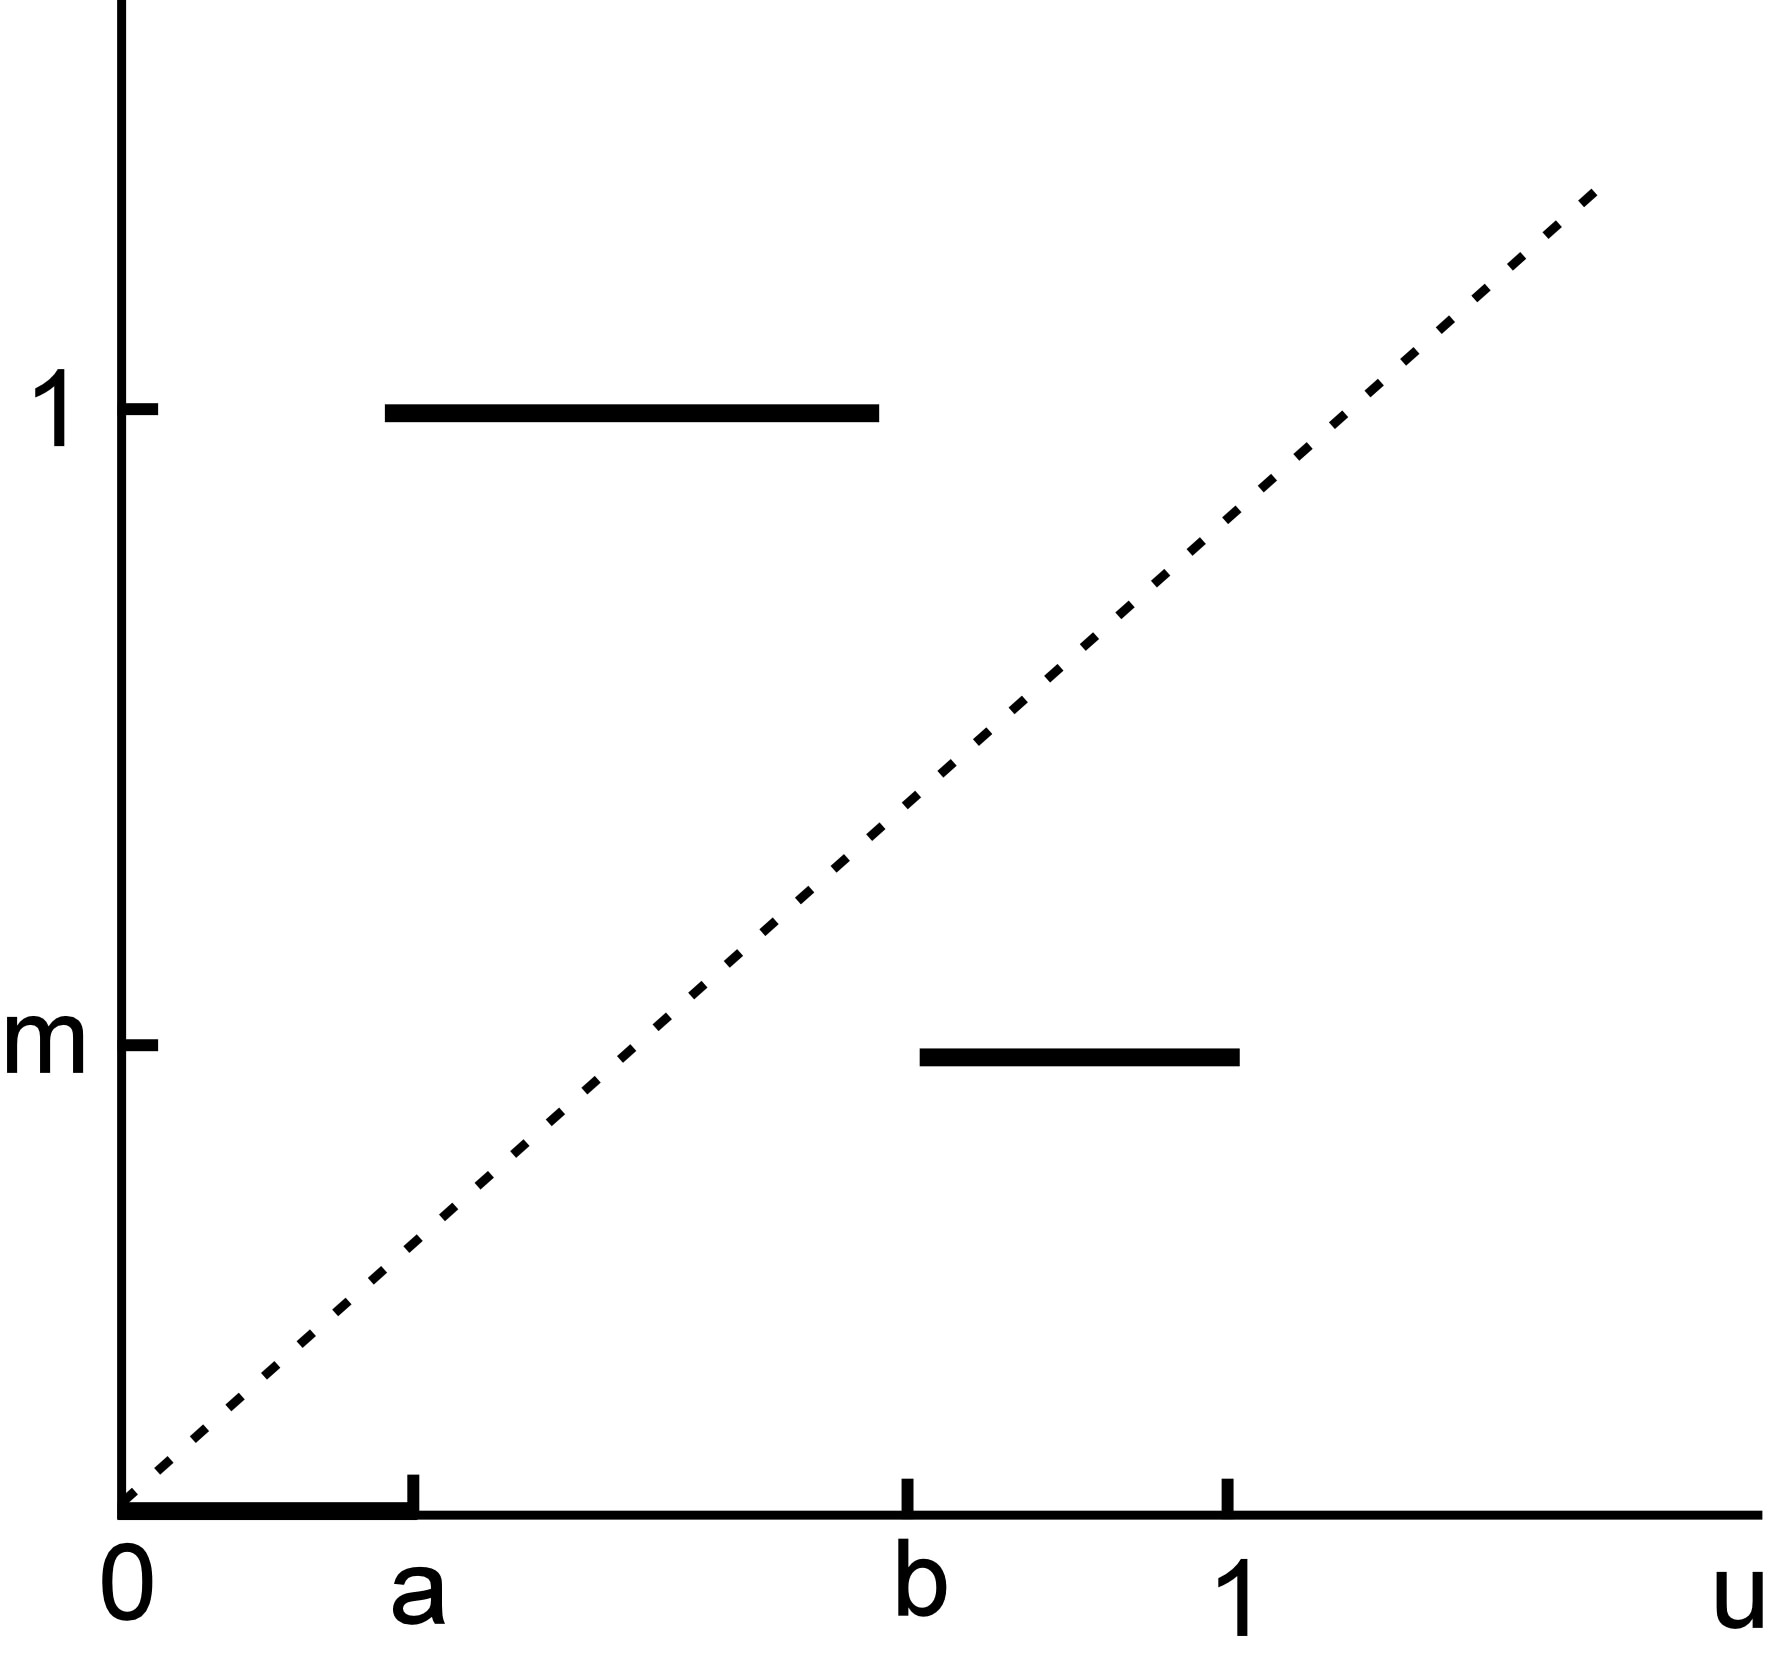
\includegraphics[width=.4\linewidth]{figures/fig1.jpg}
\end{figure}
We rigorously construct periodic traveling waves with two intermediate speed for (\ref{q}) with $g$ given by \eqref{g} and a proper dispersal kernel $k$. To the best of our knowledge, this is the first time that traveling waves with oscillating speeds have been analytically established  for scalar spatiotemporal equations with constant parameters. We also show that 
the mean traveling wave speed is  the spreading speed of 
solutions with compactly supported initial data under appropriate conditions.
 We finally conduct case studies for the Laplace kernel and uniform kernel.



\section{Results}

In this section, we present our main results about our model. Our assumptions about the dispersal kernel are summarized in the following hypothesis.

\begin{hyp}
$k(x)$ is a piecewise differentiable function satisfying
\begin{enumerate}[(H1)]
\item $k(x) \geq 0$ for all $x$, and $\int_{-\infty}^{\infty} k(x) \, dx = 1$, \label{h1}

\item $k(x)=k(-x)$ for all $x$,\label{h2}

\item $k(x)>0$ for all $x \in (-\sigma,\sigma)$ for some $0 < \sigma \leq \infty$,\label{h3}

\item  \label{h4}
for all $\lambda \in (0,1)$, for all $A,B\in\mathbb R$ with $A>B$, the expression
$$
k(x-A) - \lambda k(x-B)
$$
has $<2$ sign changes, and

\item \label{h5}
for all $\lambda \in (0,1)$, for all $A,B\in\mathbb R$ with $A>B$, the expression
$$
k(x-r-A) - \lambda k(x-r-B) - k(x+r+A) + \lambda k(x+r+B)
$$
has $<4$ sign changes for sufficiently large $r>0$.
\end{enumerate}
\end{hyp}



\subsection{Periodic traveling waves}

Let $w_1$ and $w_2$ be bounded, continuous functions defined by
\begin{equation} \label{w1}
w_1(x) :=\int_x^\infty k(y) \, dy
\end{equation}
and
\begin{equation} \label{w2}
w_2(x) := Q[w_1](x+c^*) =  \int_{-\infty}^{\infty} k(x+c^*-y) g(w_1(y)) \, dy
\end{equation}
where $c^*$ is a constant defined by
\begin{equation} \label{c}
c^* := \sup \{ x\in\mathbb R \mid w_2(x) = \a \}.
\end{equation}

\begin{thm} \label{theorem1}
Suppose $||w_2||_\infty < \b$. Let $v_n(x)$ be a sequence of functions defined by
\begin{equation}\label{ptw}
v_n(x) := \begin{cases}
w_1(x-nc^*), & n \text{ even}, \\
w_2(x-nc^*), & n \text{ odd},
\end{cases}
\end{equation}
for all $n \geq 0$. Then $v_n(x)$ is a periodic traveling wave (PTW) with mean wave speed $c^*$, and satisfies $v_{n+1}=Q[v_n]$ for all $n\geq0$.
\end{thm}



\begin{proof}
For each $i \in \{1,2\}$ we define the right inverse of $w_i$ by
\begin{equation}
\Phi_i(\ell) := \sup \{ x \in \mathbb R \mid w_i(x) = \ell \}, \quad i=1,2.
\end{equation}
Note that $\Phi_i(u)$ is finite for $0<\ell<||w_i||_\infty$, where $||w_1||_\infty=1$, and $\a<||w_2||_\infty<\b$ by the assumption of this theorem.

By the translation invariance property of $Q$, it suffices to show
\begin{equation} \label{qw1}
Q[w_1](x) = w_2(x-c^*)
\end{equation}
and
\begin{equation} \label{qw2}
Q[w_2](x) = w_1(x-c^*)
\end{equation}
for all $x \in \mathbb R$. The first equation follows immediately from definition \eqref{w2}. To prove the second, observe that $w_1$ is monotonically decreasing and satisfies $w_1(\infty)=0$ and $w_1(-\infty)=1$. Thus,
$$
g\circ w_1(x) = \begin{cases}
\m, & x < \Phi_1(\b), \\
1, & \Phi_1(\b) \leq x \leq \Phi_1(\a), \\
0, & x > \Phi_1(\a).
\end{cases}
$$
Applying the integro-difference operator yields
$$ \begin{aligned}
w_2(x-c^*) &= Q[w_1](x) \\
&= \m \int_{-\infty}^{\Phi_1(\b)} k(x-y) \, dy + \int_{\Phi_1(\b)}^{\Phi_1(\a)} k(x-y) \, dy \\
&= w_1(x-\Phi_1(\a)) - (1-\m) w_1(x-\Phi_1(\b)).
\end{aligned}$$
We can then differentiate with respect to $x$:
$$
\frac{dw_2}{dx} \Big| _{x-c^*}= - k(x-\Phi_1(\a)) + (\mtwo-\m) k(x-\Phi_1(\b)).
$$
From hypothesis \ref{h4}, $\frac{dw_2}{dx}$ has at most 1 sign change; thus, $w_2$ has at most 1 turning point. We also have $|| w_2 || _\infty <  \b$ hence $g\circ w_2(x) \in \{0, 1 \}$ for all $x$. We claim
\begin{equation} \label{gw2}
g\circ w_2(x) = \begin{cases}
1, & x \leq c^*, \\
0, & x > c^*,
\end{cases}
\end{equation}
where $c^*$ is defined by \eqref{c}. This can be shown by arguing in cases depending on the number of turning points of $w_2$.
\begin{enumerate}[{Case} 1.]
\item If $w_2$ has no turning points, then $w_2$ is monotone decreasing with $0 \leq w_2(x) \leq \m$ for all $x$. It follows by the intermediate value theorem (IVT) that $c^* = \Phi_2(\a)$ satisfies \eqref{gw2}. 

\item If $w_2$ has one turning point, say $x_0 \in \mathbb R$, then $w_2$ must be  increasing for $x<x_0$ and decreasing for $x>x_0$. It follows that $x_0$ is a global maximum, and $w_2$ is increasing on $(-\infty,x_0)$ and decreasing on $(x_0,\infty)$. We have $g(w_2(x))=1$ for $x<x_0$. By the IVT, $c^* = \Phi_2(\a)$ is the unique solution to \eqref{gw2}.
\end{enumerate}
Taking the convolution of equation \eqref{gw2} with $k(x)$ yields
$$
Q[w_2](x) \,=\, \int_{-\infty}^{c^*} k(x-y) \, dy \,=\, w_1(x-c^*).
$$
\end{proof}

\begin{figure}
\begin{tabular}{cc}
  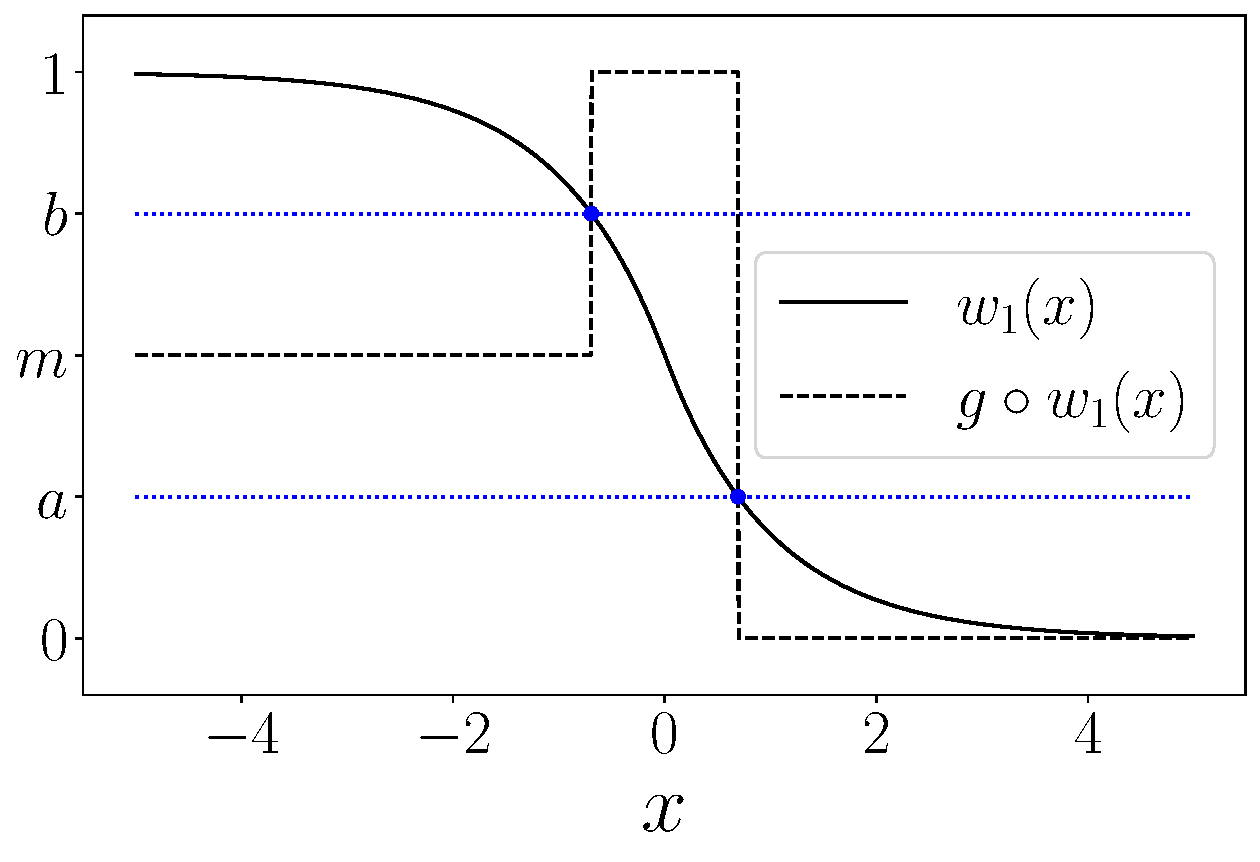
\includegraphics[width=65mm]{figures/fig7a.pdf} &   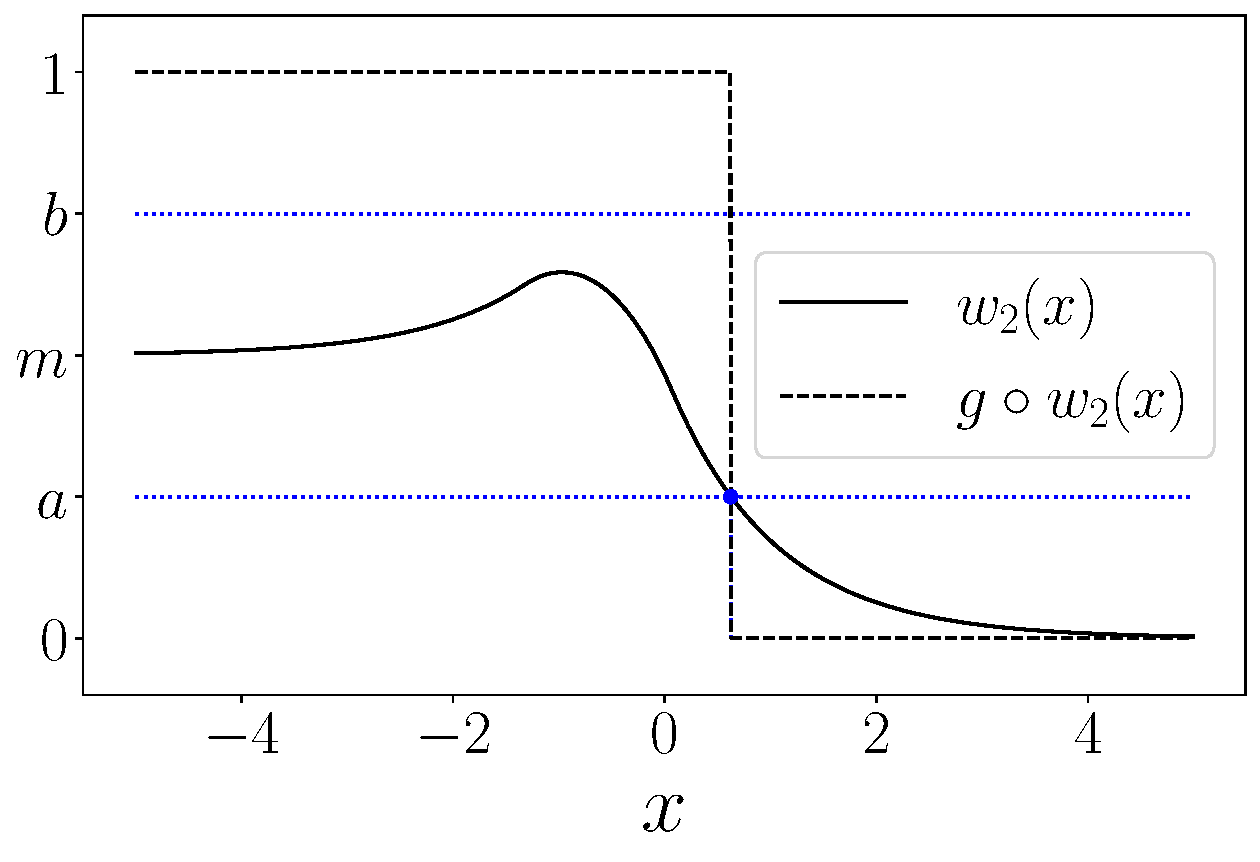
\includegraphics[width=65mm]{figures/fig7b.pdf}
\end{tabular}
\caption{Plot of $w_1(x)$ (left) and $w_2(x)$ (right) when $k(x)$ is the Laplace kernel (see Section 3). Blue points mark the intersection of the curves with the level sets $u=\a$ and $u=\b$.}
\end{figure}

Theorem \ref{theorem1} describes a rightward periodic traveling wave solution. We can define the corresponding leftward periodic traveling solution by $v_n(-x)$. This is due to the fact that $Q$ is symmetric and translation invariant.

We investigated the intermediate wave speed generated by the periodic traveling wave solution \eqref{ptw}. For this purpose, we define a sequence $\xi_n(\ell)$ depending on a fixed real number $\ell \in (0,\m)$ by

\begin{equation}
 \xi_n(\ell) = \sup \{ x \in \mathbb R : v_n(x) = \ell \}.
\end{equation}

The sequence $\xi_n$ is the rightmost intersection of the curve $u=v_n(x)$ with the horizontal line $u=\ell$. By computing the first difference of the sequence $\xi_n$, we obtain a new sequence $c_n(\ell)$ defined by
\begin{equation}
c_n(\ell) := \xi_{n+1}(\ell) - \xi_n(\ell).
\end{equation}
for $n \geq 0$.  It follows from Theorem \ref{theorem1} that $c_n(\ell)$ converges to a period-$2$ cycle for every $\ell \in (0,\m)$. Our results about the intermediate wave speed sequence is summarized in the following corollary.



\begin{cor}
The sequence $c_n(\ell)$ satisfies
\begin{equation}
c_n(\ell) = \begin{cases}
c_1^*(\ell), & n \text{ even}, \\
c_2^*(\ell), & n \text{ odd},
\end{cases}
\end{equation}
for all $\ell \in (0,\m)$, where $c_1^*(\ell)$ and $c_2^*(\ell)$ are given by
\begin{equation} \label{c1star}
c_1^*(\ell) := c^* + \Phi_1(\ell) - \Phi_2(\ell)
\end{equation}
and
\begin{equation} \label{c2star}
c_2^*(\ell) := c^* + \Phi_2(\ell) - \Phi_1(\ell).
\end{equation}
Furthermore, they satisfy the identity
\begin{equation}
c_1^*(\ell) + c_2^*(\ell) = 2c^*
\end{equation}
for all $\ell \in (0,\m)$.
\end{cor}

\begin{proof}
By Theorem \ref{theorem1}, we have
$$ \begin{aligned}
\xi_n(\ell) &= \begin{cases}
\sup\{x \in \mathbb R \mid w_1(x-nc^*) = \ell \}, & n \text{ even},\\
\sup\{x \in \mathbb R \mid w_2(x-nc^*) = \ell \}, & n \text{ odd},
\end{cases} \\
&= nc^* +  \begin{cases}
\Phi_1(\ell), & n \text{ even}, \\
\Phi_2(\ell), & n \text{ odd}.
\end{cases}
\end{aligned}
$$

Taking successive differences yields

$$ \begin{aligned}
c_n(\ell) &= \xi_n(\ell) - \xi_{n-1}(\ell) \\
&= nc^* +  \begin{cases}
\Phi_1(\ell), & n \text{ even}, \\
\Phi_2(\ell), & n \text{ odd},
\end{cases} - (n-1)c^* +  \begin{cases}
\Phi_2(u), & n \text{ even}, \\
\Phi_1(u), & n \text{ odd}
\end{cases} \\
&= c^* + \begin{cases}
\Phi_1(\ell) - \Phi_2(\ell), & n \text{ even}, \\
\Phi_2(\ell) - \Phi_1(\ell), & n \text{ odd}.
\end{cases}
\end{aligned} $$
\end{proof}

Thus, $\eqref{q}$ has a periodic traveling wave with wave profiles $w_1(x)$ and $w_2(x)$, intermediate wave speeds $c_1^*(\ell)$ and $c_2^*(\ell)$,  and average wave speed  $c^*$. Note that the intermediate wave speeds depend on the level $\ell$ at which they are measured, but their sum is given by the constant $2c^*$.

\subsection{Spreading solutions}

By applying the results of Theorem \ref{theorem1}, we were able to prove the asymptotic spreading speed of solutions with compact initial data. In particular, we showed that $c^*$ is the asymptotic spreading speed of initial data with sufficiently large weight above the Allee threshold but below the overcompensation threshold.


\begin{thm} \label{theorem2}
Suppose that the initial condition $u_0(x)$ of recurrence \eqref{q} is continuous, has compact support, satisfies $|| u_0 || _\infty < \b$, and that the set $A = \{ x \in \mathbb R : u_0(x) \geq \a \}$ is connected. If
\begin{enumerate}[i.]
\item $||w_2|| _\infty < \b$,
\item the diameter of $A$ is sufficiently large, and 
\item $c^* > 0$,
\end{enumerate}
then the sequence $u_n(x)$ spreads asymptotically with mean speed $c^*$ as $n\to\infty$.
\end{thm}

\newcommand{\what}{\tilde{w_1}}
\newcommand{\whattwo}{\tilde{w_2}}
\newcommand{\whatgen}{\tilde{w}}

\begin{proof}
We define two multivariate functions $\what,\whattwo : \mathbb R \times [0,\infty)\to\mathbb R$ by
\begin{equation}
\what(x,r) := w_1(x) - w_1(x+2r) = \int_{-2r}^{0} k(x-y) \, dy
\end{equation}
and
\begin{equation}
\whattwo(x,r) := Q[\what](x+c^*).
\end{equation}
Observe that $\what$ is symmetric with respect to $x=-r$, and $\whattwo$ is symmetric with respect to $x=-r-c^*$. This notation can be justified by observing that $\what(x,r) \to w_1(x)$ and $\whattwo(x,r)\to w_2(x)$ as $r\to\infty$ for all $x$. We also set
\begin{equation}
\phi_i(r,\ell) := \sup \{ x \in \mathbb R \mid \whatgen_i(x,r) = \ell \}, \quad i=1,2.
\end{equation}
$\phi_1$ and $\phi_2$ are the right-inverse of $\what$ and $\whattwo$, respectively. For a fixed $r>0$, the value of $\phi_i(r,\ell)$ is finite if $0 < \ell < || \whatgen_i(\cdot, r) || _\infty$, with the latter bound converging to $||w_i||_\infty$ as $r\to\infty$. They satisfy
$$
\lim_{r\to\infty} \phi_i (r,\ell) = \Phi_i(\ell) , \quad 0 < \ell < || w_i ||_\infty, \quad i=1,2.
$$

We now apply the growth function to $\what$, assuming $r$ is sufficiently large enough so that $\a < ||\what(\cdot,r)||_\infty < \b$; this is guaranteed by taking $r >  \Phi_1\left(\frac{1-a}{2}\right)$. We have
$$
g \circ \what(x,r)  = \begin{cases}
0, & x < -2r - \phi_1(r,a), \\
1, & -2r - \phi_1(r,a) < x < -2r - \phi_1(r,b), \\
\m, & -2r - \phi_1(r,b) < x < \phi_1(r,b),\\
1, & \phi_1(r,b) < x < \phi_1(r,a), \\
0, & x > \phi_1(r,a).
\end{cases} $$
Note that the above expression converes to $g \circ w_1(x)$ as $r\to\infty$. We then apply the convolution operator:
$$\begin{aligned} 
\whattwo(x-c^*,r) = Q[\what(\cdot,r)](x) &= \int_{-2r-\phi_1(r,a)}^{\phi_1(r,a)} k(x-y) \, dy - (1-\m) \int_{-2r-\phi_1(r,b)}^{\phi_1(r,b)} k(x-y) \, dy \\
&= w_1(x-\phi_1(r,a)) - (1-\m) w_1(x-\phi_1(r,b)) \\
&+ (1-\m) w_1(x+2r+\phi_1(r,b)) - w_1(x+2r+\phi_1(r,a)).
\end{aligned}$$
Computing the derivative of this expression yields
$$\begin{aligned} \label{qhatcomputation2}
\frac{d\whattwo}{dx}\Big|_{x-c^*} &= -k(x-\phi_1(r,a)) + (1-\m) k(x-\phi_1(r,b)) \\
& - (1-\m) k(x+2r+\phi_1(r,b)) + k(x+2r+\phi_1(r,a)).
\end{aligned}$$

By hypothesis \ref{h5}, the number of turning points of $\whattwo$ is at most 3 (assuming $r$ is sufficiently large). Furthermore, $\whattwo$ is symmetric around $x=-r-c^*$; thus the sign changes must come in pairs or occur exactly at $x=-r-c^*$. We can immediately exclude the cases of 0 and 2 turning points because $\whattwo$ is non-negative, vanishes at $\pm\infty$, and is not identically zero. As in the proof of Theorem \ref{theorem1}, this leaves two cases:
\begin{enumerate}[{Case} 1.]

\item If $\whattwo$ has 1 turning point, then it must occur at $x=-r-c^*$. We have $\whattwo(-r-c^*,r) = w_2(-r-c^*) - w_2(r+c^*) \to \m$ as $r \to \infty$; hence, it is sufficient to take $r$ large enough so that $|\whattwo(-r-c^*,r) - \m| < \min\{|\a-\m|,|\b-\m|\}$; it follows by the triangle inequality that $\whattwo(x,r) \leq \whattwo(-r-c^*,r) < \b$ for all $x$.

\item If $\whattwo$ has 3 turning points, then again by symmetry, they must be given by $\{-r-c^*-t, -r-c^*, -r-c^*+t\}$, for some $t>0$. We can label them in increasing order by $t_1<t_2<t_3$. It follows that $t_1$ and $t_3$ are maxima with $\whattwo(t_1,r)=\whattwo(t_3,r) \to ||w_2||_\infty$ as $r\to\infty$, and $t_2$ is a local minima with $\whattwo(t_2,r) \to \m$ as $r\to\infty$. Thus $\whattwo$ is monotone increasing on $(-\infty,t_1)\cup(t_2,t_3)$ and monotone decreasing on $(t_1,t_2)\cup(t_3,\infty)$. By taking $r$ sufficiently large, we can make $\left| \whattwo(t_1,r)-||w_2||_\infty \right| = \left| \whattwo(t_3,r)-||w_2||_\infty \right| < \left| \b-||w_2||_\infty \right| $ and $\left| \whattwo(t_2,r)-\m \right| < \left| \a-\m \right|$.
\end{enumerate}

In both cases, we have $\a \leq \whattwo(x,r) \leq \b$ on a closed interval of radius $r + c^* + \phi_2(r,a)$ and $\whattwo(x,r) < a$ elsewhere. Taking composition with $g$ yields
$$
g \circ \whattwo(x-c^*,r)  = \begin{cases}
0, & x < -2r - c^* -\phi_2(r,\a), \\
1, & -2r - c^* -\phi_2(r,\a) \leq x \leq  c^* + \phi_2(r,\a) ,\\
0, & x > c^* + \phi_2(r,\a).
\end{cases}
$$
Hence,
$$ \begin{aligned}
Q^2 [\what(\cdot,r)] (x)  &= w_1(x-c^* - \phi_2(r,a)) - w_1(x+2r+c^*+\phi_2(r,a)) 
\end{aligned} $$
Shifting the expression left by $c^*+\phi_2(r,a)$ units yields
\begin{equation} \begin{aligned} \label{appliedqtwice}
Q^2 [\what(\cdot,r)] (x+c^*+\phi_2(r,a)) 
&=  \what(x, r+c^*+\phi_2(r,\a)).
\end{aligned} \end{equation}

We are now prepared to prove the theorem using an inductive argument. Let $A$ be the level set defined in the statement of the theorem. Without loss of generality, we write $A=[-r_0,r_0]$, for some $r_0>0$. Hence
$$
g \circ u_0(x) = \begin{cases}
1, & -r_0 \leq x \leq r_0, \\
0, & \text{else}.
\end{cases}
$$
Applying the convolution operator yields
$$ \begin{aligned}
u_1(x) &= w_1(x-r_0) - w_1(x+r_0) \\
&= \what(x-r_0,r_0)
\end{aligned}
$$

Let $(r_n)_{n=0}^{\infty}$ be a sequence of real numbers satisfying
\begin{equation} \label{recurrence}
r_{n+1} = r_n + c^* + \phi_2(r_n,a).
\end{equation}

If $r_0$ is sufficiently large, we can show that $r_n$ is strictly increasing and unbounded. This is due to our assumption that $c^*>0$. Since $\phi_2(r,a)\to c^*$, it suffices to assume  $|\phi_2(r,a)-c^*|<c^*$, i.e. $r_0$ is sufficieintly large so that $\phi_2(r,a)>0$ for all $r>r_0$. Plugging this into the recurrence \eqref{recurrence} yields $r_{n+1}-r_n = c^* + \phi_2(r,a) > c^* > 0$.

This argument shows that, assuming $r_0$ is sufficiently large, equation \eqref{appliedqtwice} may be applied inductively. From the principle of induction, it follows that
$$
u_{2n+1}(x) = \what(x-r_n,r_n)
$$
for all $n \geq 0$. Knowing that $(r_n)$ is unbounded allows us to use equation \eqref{recurrence} to compute the asymptotic spreading speed as the difference of successive radii:
$$
\lim_{n\to\infty} (r_{n+1}-r_n) = \lim_{n\to\infty} (c^* + \phi_2(r_n,a)) = \lim_{r\to\infty} ( c^* + \phi_2(r,a)) = 2c^*.
$$

\end{proof}



\section{Examples}

In this section, we construct the periodic traveling wave solution for uniform and Laplace kernels, as well as compute expressions for the mean wave speed as well as intermediate wave speeds in terms of the model parameters.

\subsection{Laplace kernel} 
We applied our main results to the Laplace dispersal kernel given by
\begin{equation} \label{laplacekernel}
k(x) = \frac{1}{2} e^{-|x|}
\end{equation}

$k(x)$ is symmetric and has connected support, satisfying hypotheses \ref{h1}, \ref{h2}, and \ref{h3}. We will now prove that $k(x)$ satisfies hypothesis \ref{h5}. Let $A,B\in\mathbb R$ with $A>B$, let $\lambda \in (0,1)$, and define $f(x) = k(x-A) - \lambda k(x-B)$. For $r>0$ sufficiently large, we have
$$
f(x-r) - f(-x-r) = k(x-r-A) - \lambda k(x-r-B) - k(x+r+A) + \lambda k(x+r+B)
$$
$$=  \begin{cases}
\frac{1}{2} e^{x}\left(-e^{r+A}+me^{r+B}-me^{-r-B}+e^{-r-A}\right) , & x < -r-A, \\
\frac{1}{2}e^{-x}e^{-r-A}+\frac{1}{2}e^{x}\left(e^{-r-A}-me^{-r-B}+me^{r+B}\right) , & -r-A \leq x \leq -r-B, \\
\frac{1}{2}e^{-x}\left(-e^{-r-A}+me^{-r-B}\right)+\frac{1}{2}e^{x}\left(-me^{-r-B}+e^{-r-A}\right) , & -r-B < x < r+B, \\
\frac{1}{2}e^{-x}\left(-e^{-r-A}+me^{-r-B}-me^{r+B}\right)+\frac{1}{2}e^{x}e^{-r-A}, & r+B \leq x \leq r+A \\
e^{-x}\left(-e^{-r-A}+me^{-r-B}-me^{r+B}+e^{r+A}\right), & x > r+A.
\end{cases}
$$

$f$ is monotone on $(-\infty,-r-A)\cup(r+A,\infty)$ with $f(\pm\infty)=0$; thus it cannot have any sign changes there. On each of the intervals $[-r-A,-r-B]$, $(-r-B,r+B)$, and $[r+B,r+A]$, $f$ has the form $Ce^x+De^{-x}$. Depending on the sign of $C$ and $D$, $f$ can have either one or zero sign changes on each interval. Summing over each interval, it follows that $f$ has at most $3$ sign changes. This proves hypothesis \ref{h5}; the proof of hypothesis \ref{h4} follows a similar argument.

 Assuming $||w_2||_\infty<b$, the periodic traveling wave profiles are given by

\begin{equation} \label{w1laplace}
w_1(x) =   \begin{cases} 
1 - \frac{1}{2} e^{x}, & \text{if } x \leq 0, \\
\frac{1}{2} e^{-x}, & \text{if } x > 0,
\end{cases}
\end{equation}
and
\begin{equation} \label{w2laplace}
w_2(x-c^*) = \begin{cases}
\m + \left( \frac{1}{2}(\mtwo-\m)e^{-\Phi_1(\b)} - \frac{1}{2} e^{-\Phi_1(\a)} \right) e^x, & x < \Phi_1(\b), \\
\mtwo - \frac{1}{2} e^{-\Phi_1(\a)} e^x - \frac{1}{2} (\mtwo-\m) e^{\Phi_1(\b)}   e^{-x}, & \Phi_1(\b) \leq x \leq \Phi_1(\a), \\
\left( \frac{1}{2}e^{\Phi_1(\a)} - \frac{1}{2}(\mtwo-\m) e^{\Phi_1(\b)} \right) e^{-x}, & \Phi_1(\a) < x, 
\end{cases} \end{equation}
with
\begin{equation} \label{laplacecstar}
c^* = \begin{cases}
\frac{1}{2} \ln \left( \frac{\exp(\Phi_1(\a)) -(\mtwo-\m)\exp(\Phi_1(\b))}{2\a} \right), & \a \leq u_a, \\
\frac{1}{2} \ln \left( e^{\Phi_1(\a)} \left( \mtwo - \a + \sqrt{(\mtwo-\a)^2-(\mtwo-\m)e^{\Phi_1(\b)-\Phi_1(\a)}}\right)\right), & \ell_a < \a < \ell_b, \\
\frac{1}{2} \ln \left( \frac{2(\m-\a)}{\exp(-\Phi_1(\a))-(\mtwo-\m)\exp(-\Phi_1(\b))}\right), & \a \geq u_b.
\end{cases}
\end{equation}
$\ell_a$ and $\ell_b$ are constants given by
\begin{equation}
\ell_a = \frac{1}{2}\left(1 - (\mtwo-\m) e^{\Phi_1(\b)-\Phi_1(\a)} \right), \quad 
\ell_b = \frac{1}{2} \left( 1+\m- e^{\Phi_1(\b)-\Phi_1(\a)} \right).
\end{equation}


The formulas for $\Phi_1$ and $\Phi_2$ are given by
\begin{equation}
\Phi_1(\ell) = \begin{cases} -\ln(2\ell), &\ell\leq \frac{1}{2}, \\ \ln(2-2\ell), & \ell > \frac{1}{2}, \end{cases}
\end{equation}
and
\begin{equation}
\Phi_2(\ell) = -c^* + \begin{cases}
\ln \left( \frac{\exp(\Phi_1(\a)) -(\mtwo-\m)\exp(\Phi_1(\b))}{2\ell} \right), & \ell \leq w_2(\Phi_1(\a)), \\
\ln \left( e^{\Phi_1(\a)} \left( \mtwo - \ell+ \sqrt{(\mtwo-\ell)^2-(\mtwo-\m)e^{\Phi_1(\b)-\Phi_1(\a)}}\right)\right), & w_2(\Phi_1(\a)) < \ell < w_2(\Phi_1(\b)), \\
\ln \left( \frac{2(\m-\ell)}{\exp(-\Phi_1(\a))-(\mtwo-\m)\exp(-\Phi_1(\b))}\right), & \ell\geq w_2(\Phi_1(\b)).
\end{cases}
\end{equation}
For a more explicit formula for $c^*$, see appendix \ref{laplacespeedcalculations}. The intermediate wave speeds can be determined analytically by $c_1^*(\ell) = c^* + \Phi_1(\ell) - \Phi_2(\ell)$ and $c_2^*(\ell)=c^* + \Phi_2(\ell) - \Phi_1(\ell)$.

Figure \ref{fig:laplacewave} shows a numerical simulation of \eqref{q} with Laplace dispersal kernel showing the propagation of the periodic traveling wave solution ($1 \leq n \leq 11$). Later timepoints are colored in red, with earlier timepoints colored in green. The parameters used were $\a=0.2$, $\m=0.3$, and $\b=0.8$. Based on our spreading speed formula, we have $c^*=\frac{1}{2}\ln\frac{59}{5}$.

Figure \ref{fig:laplacecompact1} shows the time series plot for the same growth parameters and a compact initial condition with initial radius $r_0 = 0.58$, and Figure \ref{fig:laplacecompact2} shows a plot of the sequence of intermediate wave speeds for the same experiment. The dashed line represents $c^*$, which is the asymptotic average of the sequence based on Theorem \ref{theorem2}. The dotted lines represent $c_1^*$ and $c_2^*$ (evaluated at $\ell=\a$) which are the respective limit inferior and limit superior of the sequence.

While we did not analytically determine the minimal spreading speed in the proof of Theorem \ref{theorem2}, numerical simulations with  $\a=0.2$, $\m=0.3$, and $\b=0.8$ (see Figures  \ref{fig:qmu1} and \ref{fig:qmu2}) show that the shape of $\whattwo$ satisfies our assumptions for large enough $r$.


\begin{figure}[h!]
\centering
  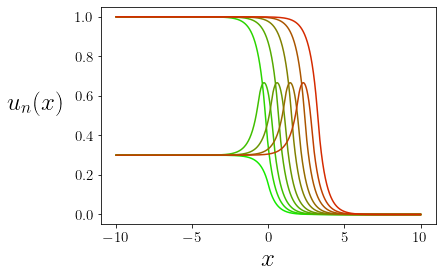
\includegraphics[scale=0.5]{figures/fig3.png}
\caption{Periodic traveling wave with Laplace dispersal kernel. Later timepoint are colored red, while earlier timepoints are colored green.}
\label{fig:laplacewave}
\end{figure}


\begin{figure}
\centering
\begin{minipage}{.5\textwidth}
  \centering
  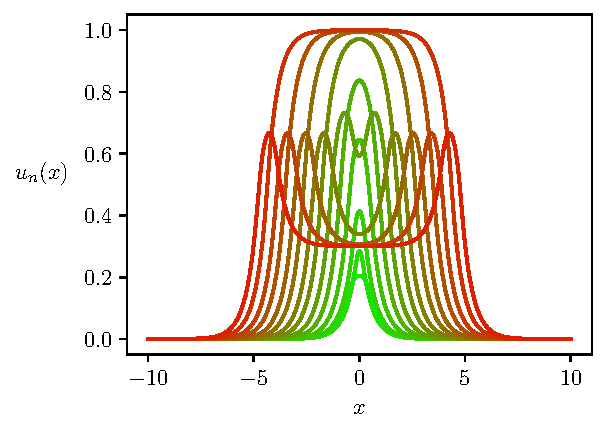
\includegraphics[width=\linewidth]{figures/fig_accelerating_wave.pdf}
\end{minipage}
\begin{minipage}{.5\textwidth}
  \centering
  \raisebox{2mm}{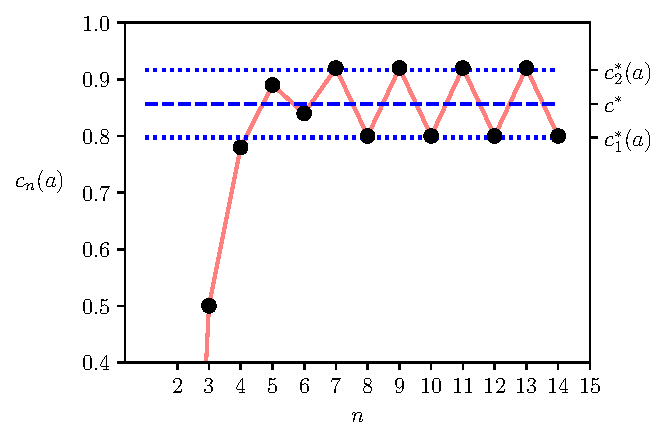
\includegraphics[width=\linewidth]{figures/fig_accelerating_wave2.pdf}}
\end{minipage}
\par
\medskip
\noindent
\begin{minipage}[t]{.49\textwidth}
  \centering
  \captionof{figure}{The first $15$ time steps of a spreading solution with Laplace dispersal kernel and compact initial data ($r_0=0.58$). }
  \label{fig:laplacecompact1}
\end{minipage}
\hfill
\begin{minipage}[t]{.49\textwidth}
  \centering
  \captionof{figure}{Time series plots of the sequence of intermediate wave speed $c_n(\ell)$. The horizontal blue lines represent the theoretical limiting values derived in Theorem \ref{theorem2}.}
  \label{fig:laplacecompact2}
\end{minipage}
\end{figure}





\begin{figure}
\centering
\begin{minipage}{.5\textwidth}
  \centering
  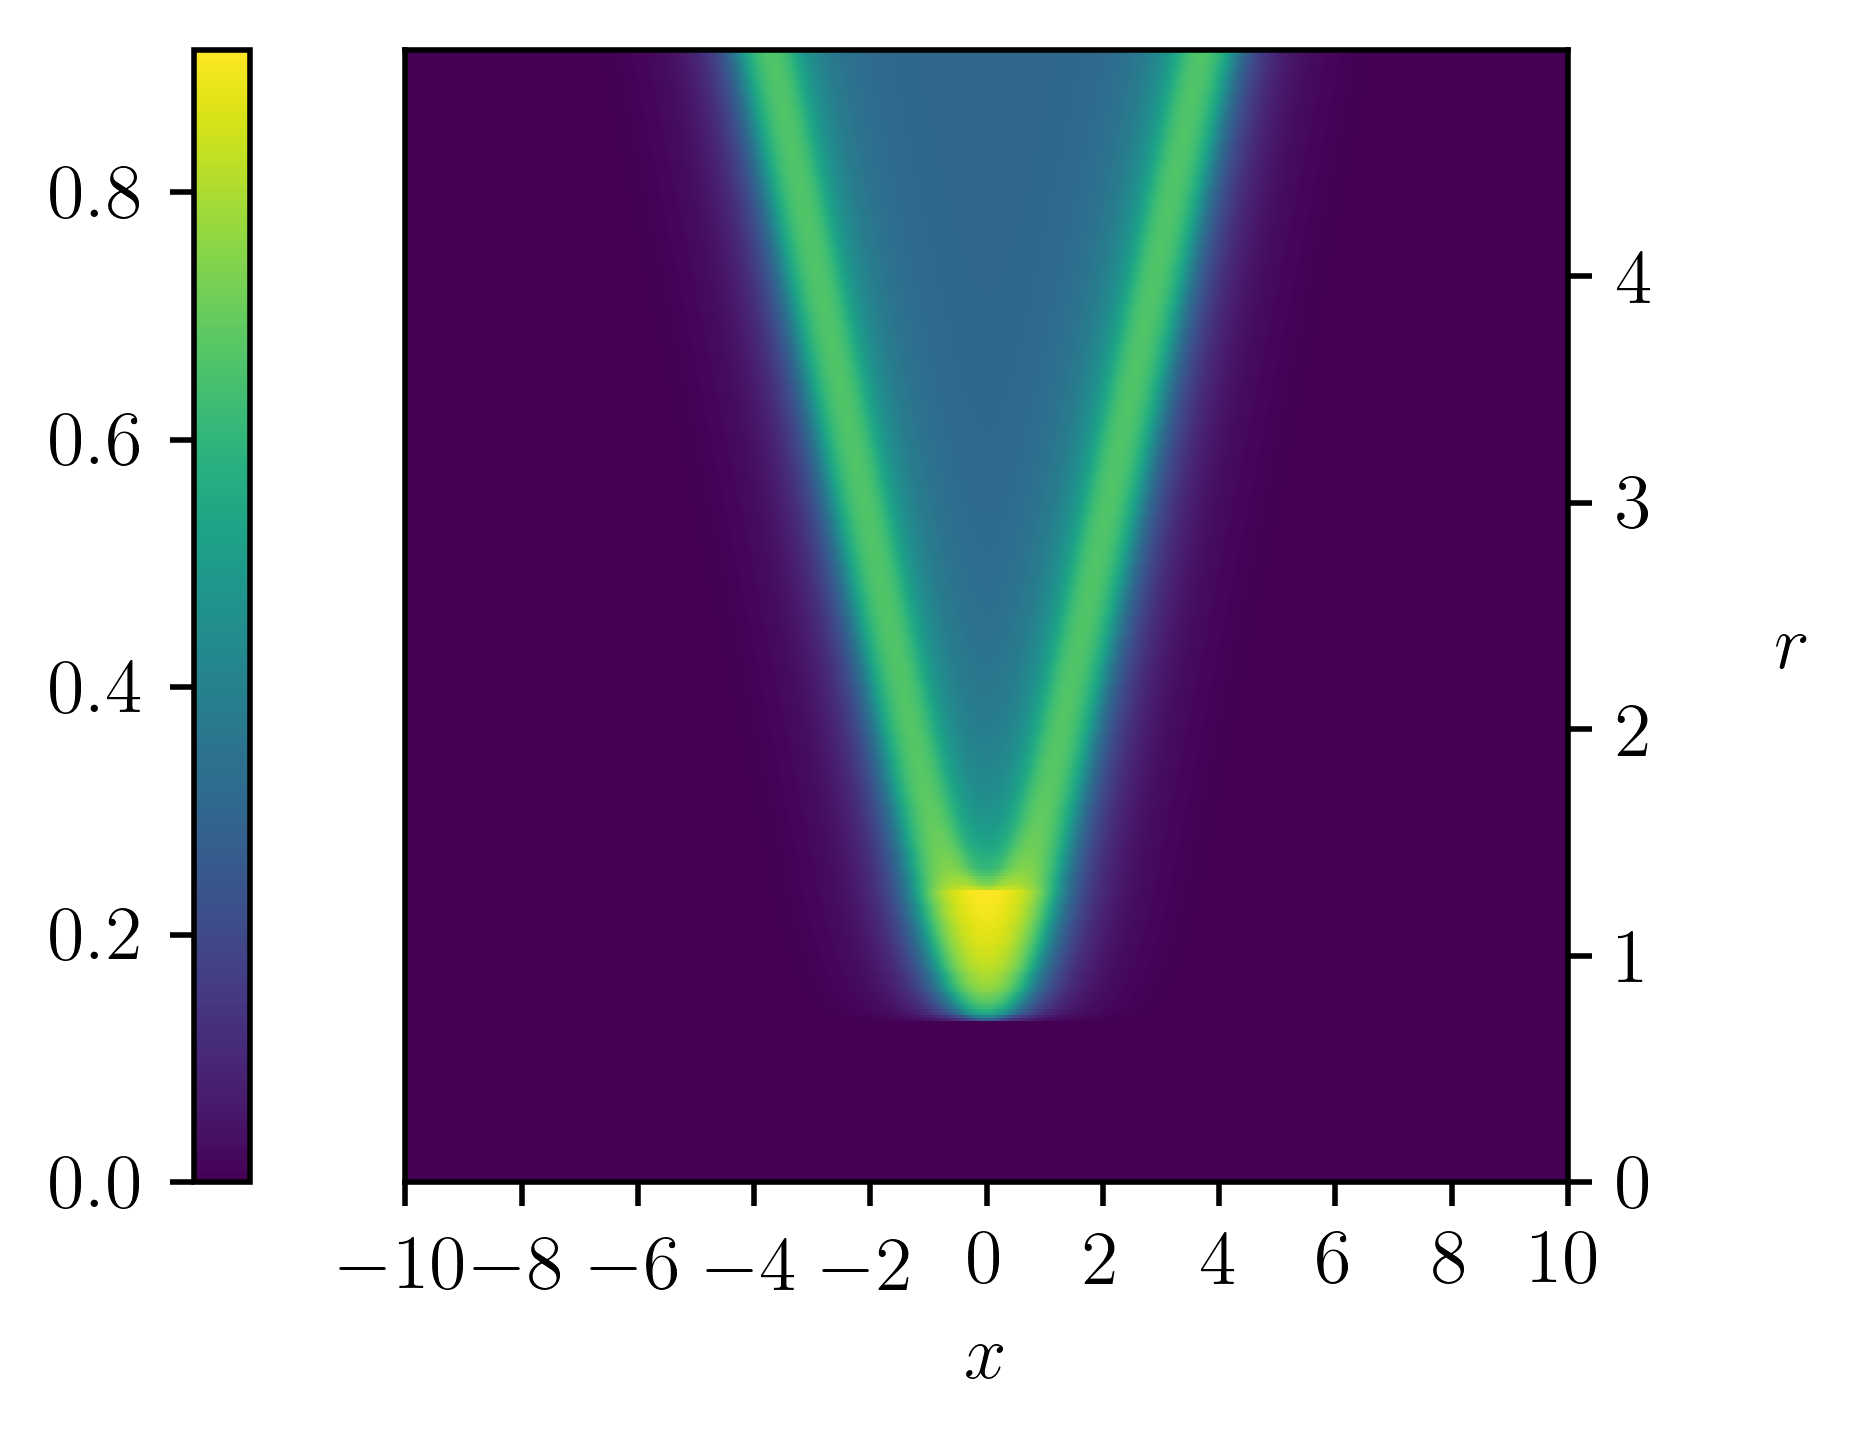
\includegraphics[width=\linewidth]{figures/fig6a.png}
\end{minipage}
\begin{minipage}{.5\textwidth}
  \centering
  \raisebox{6mm}{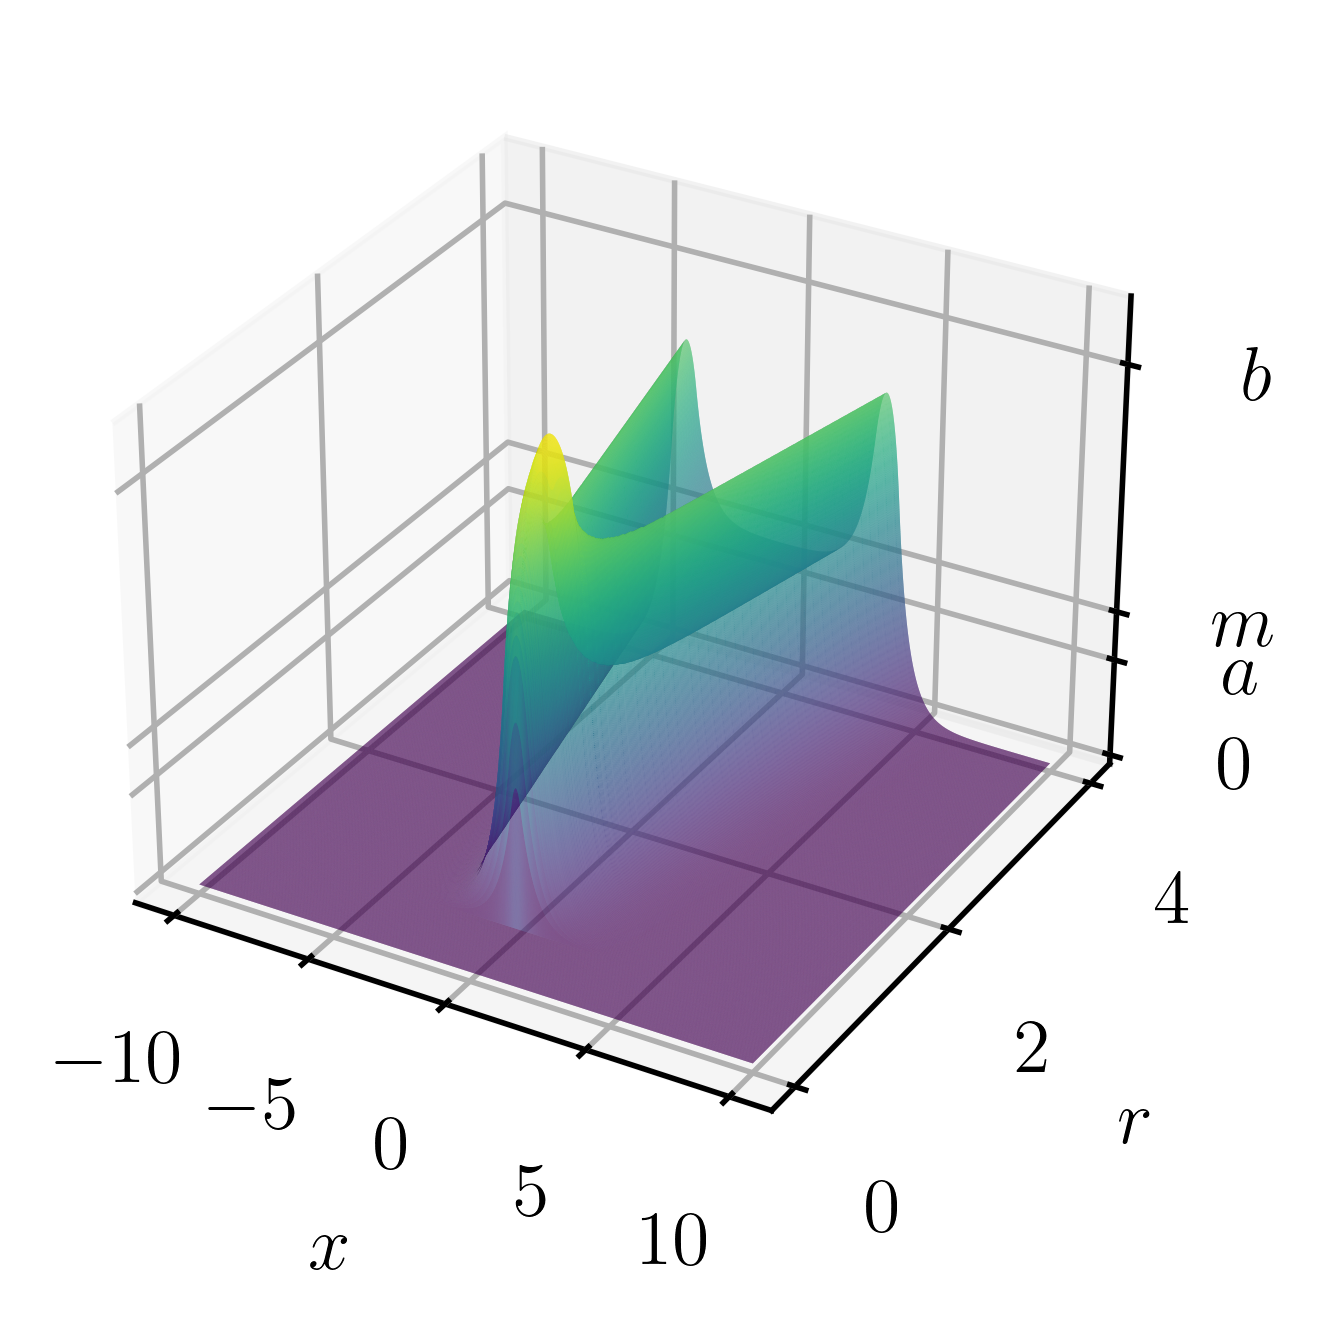
\includegraphics[width=\linewidth]{figures/fig6b.png}}
\end{minipage}
\par
\medskip
\noindent
\begin{minipage}[t]{.49\textwidth}
  \centering
  \captionof{figure}{Heatmap of $\whattwo(x-r-c^*,r)$ with Laplace dispersal kernel.}
  \label{fig:qmu1}
\end{minipage}
\hfill
\begin{minipage}[t]{.49\textwidth}
  \centering
  \captionof{figure}{Surface plot of $\whattwo(x-r-c^*,r)$ with Laplace dispersal kernel.}
  \label{fig:qmu2}
\end{minipage}
\end{figure}



\subsection{Uniform kernel}

Consider the uniform dispersal kernel given by
\begin{equation}
k(x) = \begin{cases}
\frac{1}{2}, & \text{if } |x|\leq 1, \\
0, & \text{if } |x| > 1.
\end{cases} \end{equation}
Like the previous example, $k(x)$ is symmetric around zero. We can verify hypothesis \ref{h4} by letting $A>B$ and $\lambda \in (0,1)$ and defining $f(x)=k(x-A)-\lambda k(x-B)$. There are two cases:
\begin{enumerate}[{Case} 1.]
\item If $|A-B|<2$, then
$$
f(x) = \begin{cases}
0, & x \leq B-1, \\
-\frac{\lambda}{2}, & B-1 < x \leq A-1, \\
\frac{1-\lambda}{2}, & A-1 < x < B+1, \\
\frac{1}{2}, & B+1 \leq x < A+1 \\
0, & x \geq A+1.
\end{cases}
$$

\item If $|A-B| \geq 2$, then
$$
f(x) = \begin{cases}
0, & x \leq B-1, \\
-\frac{\lambda}{2}, & B-1 < x < B+1, \\
0, & B+1 \leq x \leq  A-1, \\
\frac{1}{2}, & A-1 < x < A+1 \\
0, & x \geq A+1.
\end{cases}
$$
\end{enumerate}
In both cases, the number of sign changes is exactly 1. To extend this argument to hypothesis \ref{h5}, observe that since $k(x)$ has compact support, we have
$$
\begin{aligned}
f(x-r) - f(r-x) &= k(x-r-A) - \lambda k(x-r-B) - k(x+r+A) + \lambda k(x+r+B) \\
&=  \begin{cases}
-f(r-x), & x < -r+1, \\
0, & -r+1 \leq x \leq r-1, \\
f(x-r), & x > r-1,
\end{cases}
\end{aligned}
$$
for sufficiently large $r$. 


The alternating wave profiles are given by
\begin{equation}  \label{uniformw1}
\begin{aligned}
w_1(x) 
= \begin{cases}
1, & x \in (-\infty, -1), \\
\frac{1}{2}-\frac{1}{2}x, & x \in [-1, 1] ,\\
0, & x \in (1, \infty),
\end{cases}
\end{aligned} \end{equation}
and 
\begin{equation} \label{uniformw2}
\begin{aligned}
w_2(x+c^*)
= \begin{cases}
m,
& x \in (-\infty, -2\b), \\
\frac{1-m}{2}x + m + b - mb,
& x \in [-2\b, 
 -2\a), \\
-\frac{m}{2}x +m+b- mb-a,
& x \in [-2\a, 2-2\b), \\
-\frac{1}{2} x-a+1,
& x \in [2-2\b, 2-2\a], \\
0,
& x \in (2+2\a,\infty),
\end{cases}
\end{aligned} \end{equation}
with
\begin{equation} \label{clinear}
c^* = \begin{cases}
1 - 2a, & \text{if } a \leq b/2, \\
1 -b + \frac{b - 2a}{m}, & \text{if }a > b/2.
\end{cases}
\end{equation}

Observe that $w_2$ has a global maximum at $x=-2\a$ so that $||w_2||_\infty=m+(b-a)(1-m)$. Thus, a sufficient condition for the existence of the periodic traveling wave is $w_2(-2\a)=m+(b-a)(1-m) < \b$. 

The intermediate wave speeds are given by
\begin{equation} \begin{aligned}
c_1^*(\ell) 
&= 1-2\ell
\end{aligned}
\end{equation}
and
\begin{equation} \begin{aligned}
c_2^*(\ell) 
&= \begin{cases}
1 - 4a + 2\ell, & a \leq b/2, \\
1 - 2b + \frac{2b-4a}{m} + 2\ell, & a > b/2 ,
\end{cases}
\end{aligned} \end{equation}
for $0 < \ell < m + (b-a)(1-m)$. By evaluating the intermediate wave speeds at $\ell=\a$, it is easily seen that $c_1^*(\a)=c_2^*(\a)$ if $\a \leq \b/2$, and $|c_1^*(\a)-c_2^*(\a)|=2(2\a-\b)(\frac{1-\m}{\m})>0$ if $a>b/2$. So for $a>b/2$, the traveling wave is periodic with two different intermediate wave speeds. Furthermore, the difference between these two intermediate speeds is increasing with respect to the Allee threshold $\a$ and decreasing with respect to the overcompensation threshold $\b$.

Figure \ref{fig:uniformplot1} depicts the periodic traveling wave solution \ref{ptw} with the uniform kernel with growth parameters are $\a=0.325$, $\b=0.6$, and $\m=0.45$. The mean spreading speed can be analytically calculated as $c^*=\frac{13}{45}$. The intermediate speeds are $c_1^*(\a)=\frac{7}{20}$ and $c_2^*(\a)=\frac{41}{180}$. Figure \ref{fig:uniformplot2} demonstrates the spreading phenomena with initial domain rize $r_0=1$. Since our uniform kernel is compact with support $[-1,1]$, a sufficient lower bound on the initial domain size is $r_0 \geq 3$.


\begin{figure}
\centering
\begin{minipage}{.5\textwidth}
  \centering
  \raisebox{6mm}{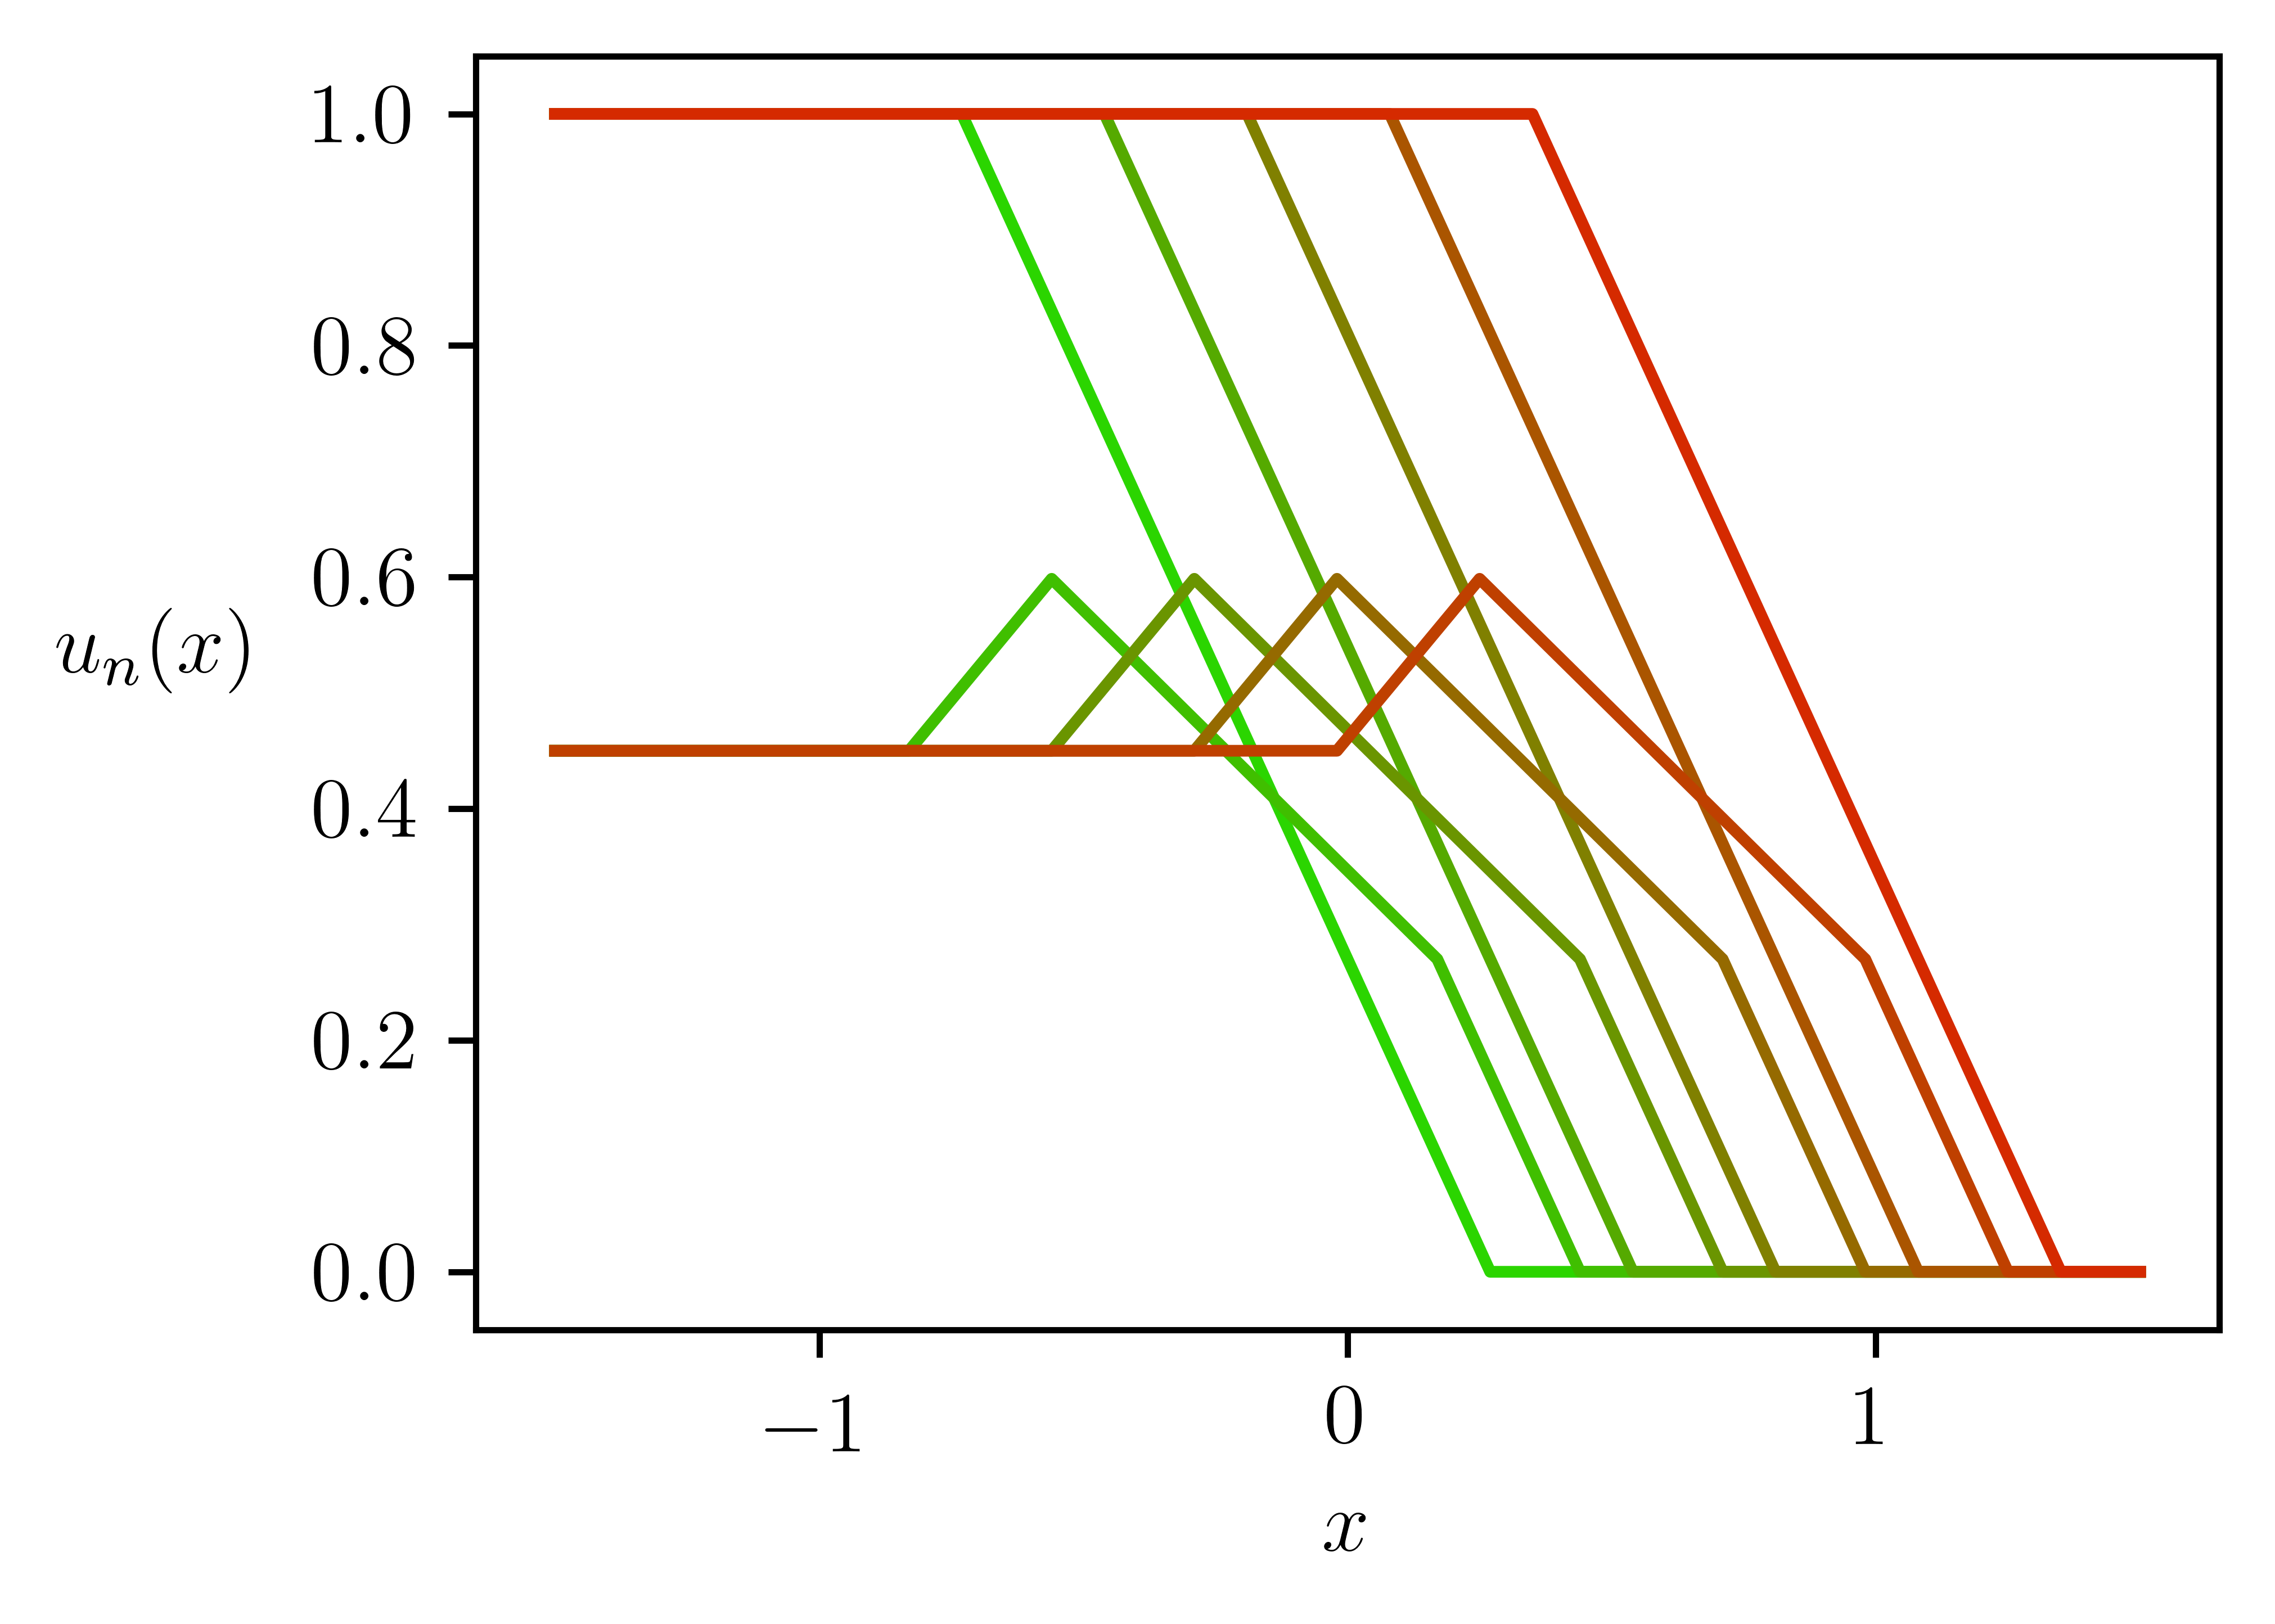
\includegraphics[width=\linewidth]{figures/fig8.png}}
\end{minipage}%
\begin{minipage}{.5\textwidth}
  \centering
  \raisebox{6mm}{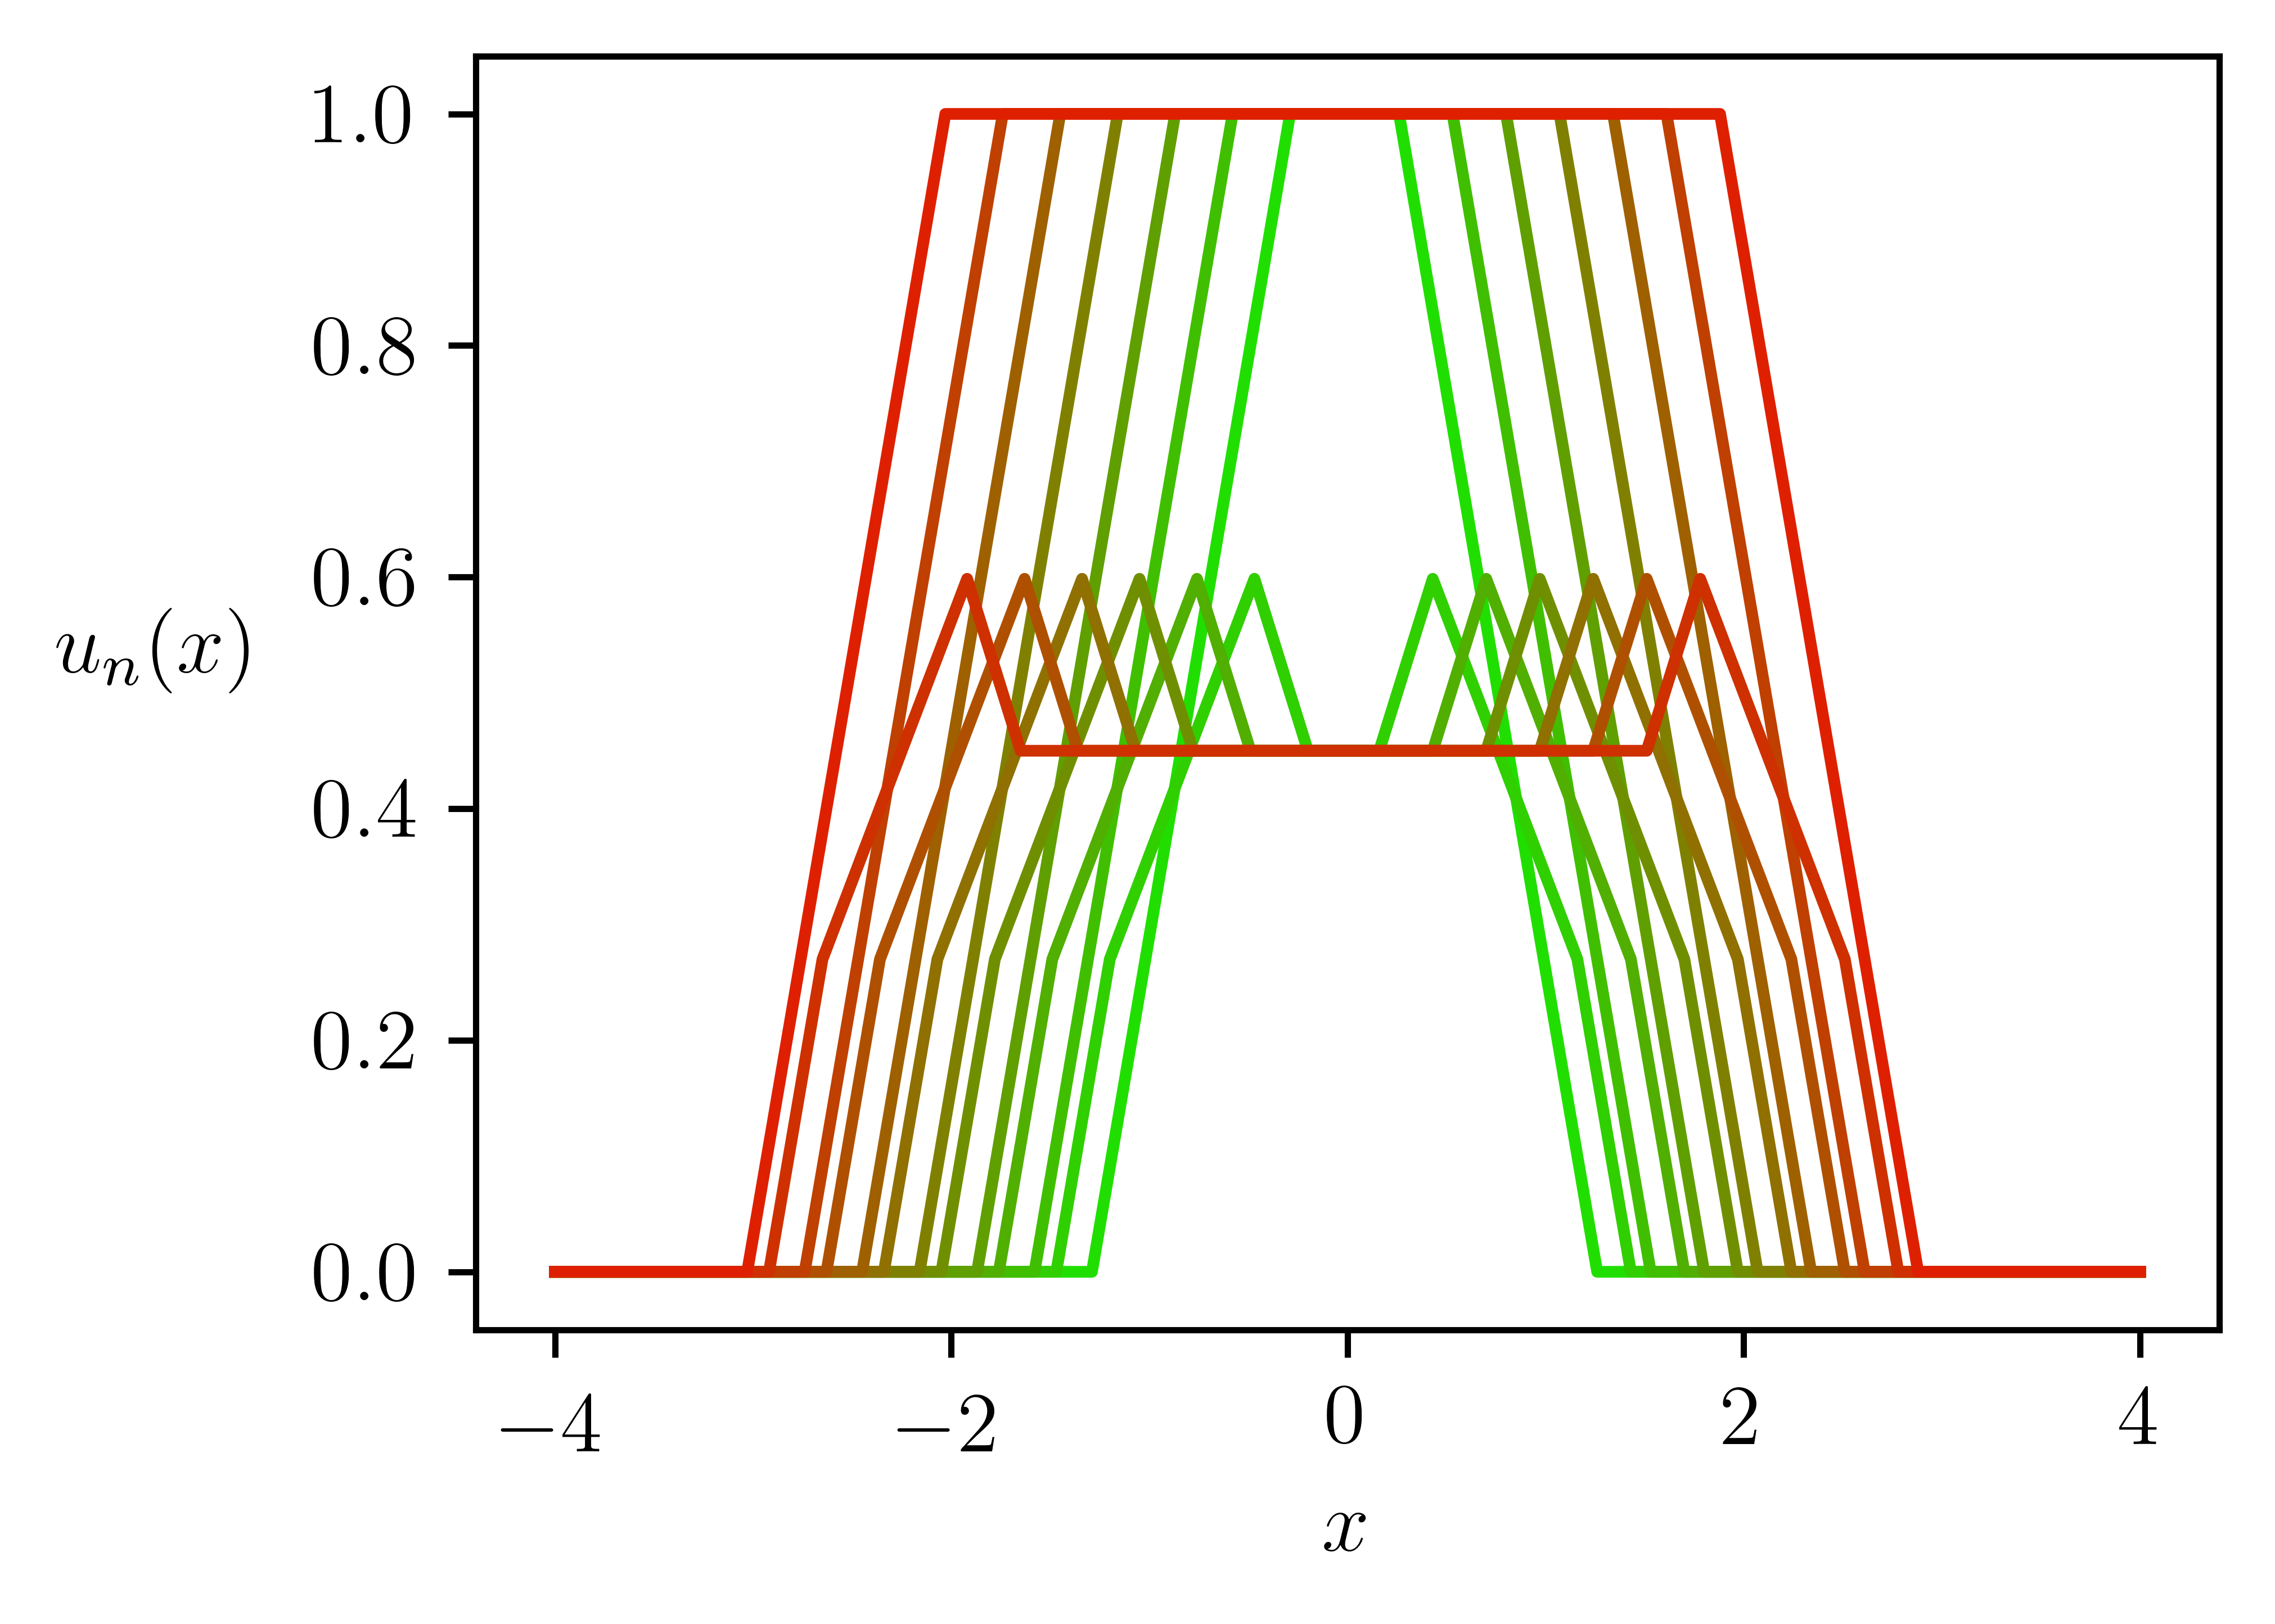
\includegraphics[width=\linewidth]{figures/fig9.png}}
\end{minipage}
\par
\medskip
\noindent
\begin{minipage}[t]{.49\textwidth}
  \centering
  \captionof{figure}{Periodic traveling wave solution with uniform dispersal kernel.}
  \label{fig:uniformplot1}
\end{minipage}%
\hfill
\begin{minipage}[t]{.49\textwidth}
  \centering
  \captionof{figure}{Spreading behavior of the uniform kernel.}
  \label{fig:uniformplot2}
\end{minipage}
\end{figure}


\begin{thebibliography}{9}
\bibitem{all}  W. C. Allee. 1931. Animal Aggregations. A Study on
General Sociology. University of Chicago Press, Chicago, IL.


%\bibitem{htw90} D. P. Hardin, P. Tak$\acute{\mbox{a}}\check{\mbox{c}}$, and G. F. Webb. 1990. Dispersion population %models discrete in time and
%continuous in space. J. Math. Biol. {\bf 28}: 1-20.

\bibitem{hh} A. Hastings and K. Higgins. 1994. Persistence of transients in spatially
structured ecological models. Science {\bf 263}: 1133-1136.

%\bibitem{hz} S.-B. Hsu and X.-Q. Zhao. 2008. Spreading speeds and traveling waves for nonmonotone integrodifference equations. SIAM J. Math. Anal. {\bf} 40: 776–789


\bibitem{ks} M. Kot and W. M. Schaffer. 1986.  Discrete-time growth-dispersal models.
Math. Biosci. {\bf 80}: 109-136.


\bibitem{kot89} M. Kot. 1989. Diffusion-driven period doubling bifurcations.
Biosystems {\bf 22}: 279-287.


\bibitem{kot92} M. Kot. 1992. Discrete-time traveling waves:
Ecological examples. J. Math. Biol. {\bf 30}: 413-436.


\bibitem{kot1} M. Kot, M. A. Lewis, and P. van den Driessche. 1996. Dispersal data and the spread of invading
organisms. Ecology {\bf 77}: 2027-2042.


%\bibitem{kot2} M. Kot, J. Medlock, T. Reluga, and D. B. Walton. 2004. Stochasticity, invasions, and branching random walks. Theor. Popul. Biol. {\bf 66}: 175-184.


%\bibitem{li09} B. Li, M. A. Lewis, and H. F. Weinberger. 2009.  Existence of traveling waves for integral recursions with nonmonotone growth functions. J. Math. Biol. {\bf 58}: 323-338.


\bibitem{kotbook} M. Kot. 2001. Elements of Mathematical Ecology.
Cambridge University Press. Cambridge, United Kingdom.

\bibitem{lui82a} R. Lui. 1982. A nonlinear integral operator arising from a model in population
genetics. I. Monotone initial data. SIAM. J. Math. Anal. {\bf 13}:
913-937.

\bibitem{lui82b} R. Lui. 1982. A nonlinear integral operator arising from a model in population
genetics. II. Initial data with compact support. SIAM. J. Math.
Anal. {\bf 13}: 938-953.

\bibitem{lui83} R. Lui. 1983. Existence and stability of traveling wave solutions of a nonlinear
integral operator. J. Math. Biol. {\bf 16}:199-220.

\bibitem{lut}
F. Lutscher. 2019. Integrodifference Equations in Spatial Ecology.  Springer.


\bibitem{nkl} M. Neubert, M. Kot, and M. A. Lewis. 1995. Dispersal and pattern formation in a
discrete-time predator-prey model. Theor. Pop. Biol. {\bf 48}
: 7-43.

\bibitem{otto} G. Otto. 2017. Non-spreading Solutiona in a Integro-Difference Model Incorporating Allee and Overcompensation Effects. Ph. D thesis, University of Louisville.

\bibitem{slatkin} M. Slatkin. 1973. Gene flow and selection in a cline.
Genetice {\bf 75}: 733-756.



\bibitem{pnas} L. L. Sullivan, B. Li, T. E. X. Miller, M. G. Neubert, and A. K. Shaw. 2017.
Density dependence in demography and dispersal generates fluctuating invasion speeds. Proc. Natl. Acad. Sci. USA {\bf
114}: 5053-5058.


\bibitem{wang} M. H. Wang, M. Kot, and M. G. Neubert. 2002. Integrodifference equations, Allee effects, and
invasions. J. Math. Biol. {\bf 44}: 150-168.

\bibitem{w78} H. F. Weinberger. 1978. Asymptotic behavior of a model in  population genetics,
in Nonlinear Partial Differential Equations  and Applications, ed.
J. M. Chadam. Lecture Notes in Mathematics {\bf 648}: 47-96.
Springer-Verlag, Berlin.

\bibitem{wein82} H. F.  Weinberger. 1982. Long-time beahvior of a class of biological models. SIAM. J.
Math. Anal. {\bf 13}: 353-396.

\end{thebibliography}


\appendix

\section{Appendix}



\begin{prop}\label{laplacespeedcalculations}
The critical spreading speed $c^*$ for the Laplace kernel falls into one of three cases:
\begin{enumerate}[{Case} 1.]

\item $\a\leq\frac{1}{2}$, $\b\leq\frac{1}{2}$:
$$
c^* = \begin{cases}
\frac{1}{2} \ln \left( \frac{\b-\a(1-\m)}{4\a^2\b} \right), & \a < \frac{\b-\a(1-\m)}{2\b}, \\
\frac{1}{2} \ln \left( \frac{1-\a + \sqrt{(1-\a)^2 - \frac{\a(1-\m)}{\b}}}{2\a} \right), & \frac{\b-\a(1-\m)}{2\b} \leq \a \leq \frac{\b(1+\m)-\a}{2\b}, \\
\frac{1}{2} \ln \left( \frac{\a-\m}{\b(1-\m)-\a}\right), & \a > \frac{\b(1+\m)-\a}{2\b}.
\end{cases}
$$


\item $\a\leq\frac{1}{2}$, $\b>\frac{1}{2}$:
$$
c^* = \begin{cases}
\frac{1}{2} \ln \left( \frac{1-4\a(1-\m)(1-\b)}{4\a^2} \right), & a<\frac{1-4\a(1-\m)(1-\b)}{2}, \\
\frac{1}{2} \ln \left( \frac{1-\a + \sqrt{(1-\a)^2 - 4\a(1-\m)(1-\b)}}{2\a} \right), & \frac{1-4\a(1-\m)(1-\b)}{2}\leq\a\leq\frac{1+\m-4\a(1-\b)}{2}, \\
\frac{1}{2} \ln \left( \frac{4(\a-\m)(1-\b)}{1-\m-4\a(1-\b)}\right), & \a>\frac{1+\m-4\a(1-\b)}{2}.
\end{cases}
$$


\item $\a>\frac{1}{2}$, $\b>\frac{1}{2}$:
$$
c^* = \begin{cases}
\frac{1}{2} \ln \left( \frac{1-\a-(1-\m)(1-\b)}{\a} \right), & \a<\frac{1-\a-(1-\m)(1-\b)}{2(1-\a)}, \\
\frac{1}{2} \ln \Big( 2(1-\a)\left[1-\a + \sqrt{\frac{(1-\a)^3-(1-\m)(1-\b) }{1-\a}}\right] \Big), & \frac{1-\a-(1-\m)(1-\b)}{2(1-\a)}\leq\a\leq\frac{\b-1+\m(1-\a)}{2(1-\a)}, \\
\frac{1}{2} \ln \left( \frac{4(\m-\a)(1-\a)(1-\b)}{1-\b+\m(1-\a)}\right), & \a>\frac{\b-1+\m(1-\a)}{2(1-\a)}.
\end{cases}
$$

\end{enumerate}
\end{prop}
\end{document}

